\documentclass[]{article}
\usepackage{lmodern}
\usepackage{amssymb,amsmath}
\usepackage{ifxetex,ifluatex}
\usepackage{fixltx2e} % provides \textsubscript
\ifnum 0\ifxetex 1\fi\ifluatex 1\fi=0 % if pdftex
  \usepackage[T1]{fontenc}
  \usepackage[utf8]{inputenc}
\else % if luatex or xelatex
  \ifxetex
    \usepackage{mathspec}
  \else
    \usepackage{fontspec}
  \fi
  \defaultfontfeatures{Ligatures=TeX,Scale=MatchLowercase}
\fi
% use upquote if available, for straight quotes in verbatim environments
\IfFileExists{upquote.sty}{\usepackage{upquote}}{}
% use microtype if available
\IfFileExists{microtype.sty}{%
\usepackage{microtype}
\UseMicrotypeSet[protrusion]{basicmath} % disable protrusion for tt fonts
}{}
\usepackage[margin=1in]{geometry}
\usepackage{hyperref}
\hypersetup{unicode=true,
            pdftitle={随机模拟方法与应用导论 作业三},
            pdfauthor={陈稼霖 45875852},
            pdfborder={0 0 0},
            breaklinks=true}
\urlstyle{same}  % don't use monospace font for urls
\usepackage{color}
\usepackage{fancyvrb}
\newcommand{\VerbBar}{|}
\newcommand{\VERB}{\Verb[commandchars=\\\{\}]}
\DefineVerbatimEnvironment{Highlighting}{Verbatim}{commandchars=\\\{\}}
% Add ',fontsize=\small' for more characters per line
\usepackage{framed}
\definecolor{shadecolor}{RGB}{248,248,248}
\newenvironment{Shaded}{\begin{snugshade}}{\end{snugshade}}
\newcommand{\AlertTok}[1]{\textcolor[rgb]{0.94,0.16,0.16}{#1}}
\newcommand{\AnnotationTok}[1]{\textcolor[rgb]{0.56,0.35,0.01}{\textbf{\textit{#1}}}}
\newcommand{\AttributeTok}[1]{\textcolor[rgb]{0.77,0.63,0.00}{#1}}
\newcommand{\BaseNTok}[1]{\textcolor[rgb]{0.00,0.00,0.81}{#1}}
\newcommand{\BuiltInTok}[1]{#1}
\newcommand{\CharTok}[1]{\textcolor[rgb]{0.31,0.60,0.02}{#1}}
\newcommand{\CommentTok}[1]{\textcolor[rgb]{0.56,0.35,0.01}{\textit{#1}}}
\newcommand{\CommentVarTok}[1]{\textcolor[rgb]{0.56,0.35,0.01}{\textbf{\textit{#1}}}}
\newcommand{\ConstantTok}[1]{\textcolor[rgb]{0.00,0.00,0.00}{#1}}
\newcommand{\ControlFlowTok}[1]{\textcolor[rgb]{0.13,0.29,0.53}{\textbf{#1}}}
\newcommand{\DataTypeTok}[1]{\textcolor[rgb]{0.13,0.29,0.53}{#1}}
\newcommand{\DecValTok}[1]{\textcolor[rgb]{0.00,0.00,0.81}{#1}}
\newcommand{\DocumentationTok}[1]{\textcolor[rgb]{0.56,0.35,0.01}{\textbf{\textit{#1}}}}
\newcommand{\ErrorTok}[1]{\textcolor[rgb]{0.64,0.00,0.00}{\textbf{#1}}}
\newcommand{\ExtensionTok}[1]{#1}
\newcommand{\FloatTok}[1]{\textcolor[rgb]{0.00,0.00,0.81}{#1}}
\newcommand{\FunctionTok}[1]{\textcolor[rgb]{0.00,0.00,0.00}{#1}}
\newcommand{\ImportTok}[1]{#1}
\newcommand{\InformationTok}[1]{\textcolor[rgb]{0.56,0.35,0.01}{\textbf{\textit{#1}}}}
\newcommand{\KeywordTok}[1]{\textcolor[rgb]{0.13,0.29,0.53}{\textbf{#1}}}
\newcommand{\NormalTok}[1]{#1}
\newcommand{\OperatorTok}[1]{\textcolor[rgb]{0.81,0.36,0.00}{\textbf{#1}}}
\newcommand{\OtherTok}[1]{\textcolor[rgb]{0.56,0.35,0.01}{#1}}
\newcommand{\PreprocessorTok}[1]{\textcolor[rgb]{0.56,0.35,0.01}{\textit{#1}}}
\newcommand{\RegionMarkerTok}[1]{#1}
\newcommand{\SpecialCharTok}[1]{\textcolor[rgb]{0.00,0.00,0.00}{#1}}
\newcommand{\SpecialStringTok}[1]{\textcolor[rgb]{0.31,0.60,0.02}{#1}}
\newcommand{\StringTok}[1]{\textcolor[rgb]{0.31,0.60,0.02}{#1}}
\newcommand{\VariableTok}[1]{\textcolor[rgb]{0.00,0.00,0.00}{#1}}
\newcommand{\VerbatimStringTok}[1]{\textcolor[rgb]{0.31,0.60,0.02}{#1}}
\newcommand{\WarningTok}[1]{\textcolor[rgb]{0.56,0.35,0.01}{\textbf{\textit{#1}}}}
\usepackage{graphicx,grffile}
\makeatletter
\def\maxwidth{\ifdim\Gin@nat@width>\linewidth\linewidth\else\Gin@nat@width\fi}
\def\maxheight{\ifdim\Gin@nat@height>\textheight\textheight\else\Gin@nat@height\fi}
\makeatother
% Scale images if necessary, so that they will not overflow the page
% margins by default, and it is still possible to overwrite the defaults
% using explicit options in \includegraphics[width, height, ...]{}
\setkeys{Gin}{width=\maxwidth,height=\maxheight,keepaspectratio}
\IfFileExists{parskip.sty}{%
\usepackage{parskip}
}{% else
\setlength{\parindent}{0pt}
\setlength{\parskip}{6pt plus 2pt minus 1pt}
}
\setlength{\emergencystretch}{3em}  % prevent overfull lines
\providecommand{\tightlist}{%
  \setlength{\itemsep}{0pt}\setlength{\parskip}{0pt}}
\setcounter{secnumdepth}{0}
% Redefines (sub)paragraphs to behave more like sections
\ifx\paragraph\undefined\else
\let\oldparagraph\paragraph
\renewcommand{\paragraph}[1]{\oldparagraph{#1}\mbox{}}
\fi
\ifx\subparagraph\undefined\else
\let\oldsubparagraph\subparagraph
\renewcommand{\subparagraph}[1]{\oldsubparagraph{#1}\mbox{}}
\fi

%%% Use protect on footnotes to avoid problems with footnotes in titles
\let\rmarkdownfootnote\footnote%
\def\footnote{\protect\rmarkdownfootnote}

%%% Change title format to be more compact
\usepackage{titling}

% Create subtitle command for use in maketitle
\providecommand{\subtitle}[1]{
  \posttitle{
    \begin{center}\large#1\end{center}
    }
}

\setlength{\droptitle}{-2em}

  \title{随机模拟方法与应用导论 作业三}
    \pretitle{\vspace{\droptitle}\centering\huge}
  \posttitle{\par}
    \author{陈稼霖 45875852}
    \preauthor{\centering\large\emph}
  \postauthor{\par}
      \predate{\centering\large\emph}
  \postdate{\par}
    \date{2019-10-01}

\usepackage[UTF8]{ctex}

\begin{document}
\maketitle

\hypertarget{relating-age-and-wage-in-the-twins-dataset}{%
\section{3.5 (Relating age and wage in the twins
dataset)}\label{relating-age-and-wage-in-the-twins-dataset}}

The variables \texttt{AGE} and \texttt{HRWAGEL} contain the age (in
years) and hourly wage (in dollars) of twin 1.

\begin{enumerate}
\def\labelenumi{\alph{enumi}.}
\item
  Using two applications of the \texttt{cut} function, create a
  categorized version of \texttt{AGE} using the breakpoints \(30\),
  \(40\), and \(50\), and a categorized version of \texttt{HRWAGEL}
  using the same breakpoints as in Section 3.3.
\item
  Using the categorized versions of AGE and HRWAGEL, construct a
  contingency table of the two variables using the function
  \texttt{table}.
\item
  Use the \texttt{prop.table} function to find the proportions of twins
  in each age class that have the different wage groups.
\item
  Construct a suitable graph to show how the wage distribution depends
  on the age of the twin.
\item
  Use the conditional proportions in part (c) and the graph in part (d)
  to explain the relationship between age and wage of the twins.
\end{enumerate}

\begin{enumerate}
\def\labelenumi{\alph{enumi}.}
\tightlist
\item
  首先读取数据文件\texttt{twins.dat.txt},用\texttt{cut}函数根据断点\(30\),\(40\)和\(50\)分割变量\texttt{AGE}并展示结果
\end{enumerate}

\begin{Shaded}
\begin{Highlighting}[]
\NormalTok{twn =}\StringTok{ }\KeywordTok{read.table}\NormalTok{(}\StringTok{'twins.dat.txt'}\NormalTok{,}\DataTypeTok{header =} \OtherTok{TRUE}\NormalTok{,}\DataTypeTok{sep =} \StringTok{','}\NormalTok{,}\DataTypeTok{na.strings =} \StringTok{'.'}\NormalTok{)}
\NormalTok{c.age =}\StringTok{ }\KeywordTok{cut}\NormalTok{(twn}\OperatorTok{$}\NormalTok{AGE,}\DataTypeTok{breaks =} \KeywordTok{c}\NormalTok{(}\DecValTok{0}\NormalTok{,}\DecValTok{30}\NormalTok{,}\DecValTok{40}\NormalTok{,}\DecValTok{50}\NormalTok{,}\DecValTok{80}\NormalTok{))}
\NormalTok{c.age}
\end{Highlighting}
\end{Shaded}

\begin{verbatim}
##   [1] (30,40] (50,80] (40,50] (30,40] (30,40] (50,80] (30,40] (50,80]
##   [9] (0,30]  (40,50] (50,80] (30,40] (30,40] (40,50] (30,40] (30,40]
##  [17] (0,30]  (0,30]  (30,40] (30,40] (0,30]  (0,30]  (30,40] (0,30] 
##  [25] (0,30]  (30,40] (30,40] (0,30]  (40,50] (40,50] (50,80] (0,30] 
##  [33] (50,80] (30,40] (50,80] (40,50] (30,40] (0,30]  (30,40] (50,80]
##  [41] (0,30]  (0,30]  (30,40] (40,50] (0,30]  (40,50] (50,80] (30,40]
##  [49] (50,80] (30,40] (50,80] (0,30]  (30,40] (50,80] (50,80] (40,50]
##  [57] (0,30]  (0,30]  (0,30]  (0,30]  (50,80] (50,80] (40,50] (30,40]
##  [65] (0,30]  (30,40] (50,80] (0,30]  (30,40] (30,40] (30,40] (30,40]
##  [73] (30,40] (30,40] (30,40] (0,30]  (30,40] (30,40] (40,50] (30,40]
##  [81] (40,50] (30,40] (0,30]  (40,50] (50,80] (0,30]  (50,80] (40,50]
##  [89] (0,30]  (50,80] (50,80] (50,80] (40,50] (30,40] (50,80] (0,30] 
##  [97] (30,40] (50,80] (40,50] (0,30]  (50,80] (0,30]  (50,80] (40,50]
## [105] (30,40] (40,50] (30,40] (0,30]  (30,40] (30,40] (30,40] (30,40]
## [113] (50,80] (30,40] (0,30]  (40,50] (30,40] (0,30]  (0,30]  (40,50]
## [121] (50,80] (50,80] (30,40] (30,40] (30,40] (30,40] (30,40] (40,50]
## [129] (40,50] (30,40] (30,40] (0,30]  (0,30]  (0,30]  (40,50] (30,40]
## [137] (0,30]  (30,40] (0,30]  (40,50] (40,50] (50,80] (40,50] (0,30] 
## [145] (30,40] (30,40] (0,30]  (50,80] (50,80] (50,80] (50,80] (0,30] 
## [153] (50,80] (0,30]  (30,40] (0,30]  (0,30]  (50,80] (40,50] (30,40]
## [161] (40,50] (30,40] (50,80] (0,30]  (30,40] (50,80] (30,40] (0,30] 
## [169] (0,30]  (30,40] (0,30]  (30,40] (40,50] (0,30]  (30,40] (40,50]
## [177] (0,30]  (30,40] (40,50] (0,30]  (40,50] (0,30]  (0,30] 
## Levels: (0,30] (30,40] (40,50] (50,80]
\end{verbatim}

然后用\texttt{cut}函数根据3.3节中的断点---------\texttt{0,7,13,20,150}---------分割变量\texttt{HRWAGEL}并展示结果

\begin{Shaded}
\begin{Highlighting}[]
\NormalTok{c.wage =}\StringTok{ }\KeywordTok{cut}\NormalTok{(twn}\OperatorTok{$}\NormalTok{HRWAGEL,}\DataTypeTok{breaks =} \KeywordTok{c}\NormalTok{(}\DecValTok{0}\NormalTok{,}\DecValTok{7}\NormalTok{,}\DecValTok{13}\NormalTok{,}\DecValTok{20}\NormalTok{,}\DecValTok{150}\NormalTok{))}
\NormalTok{c.wage}
\end{Highlighting}
\end{Shaded}

\begin{verbatim}
##   [1] (7,13]   (7,13]   (7,13]   (13,20]  (13,20]  <NA>     (7,13]  
##   [8] <NA>     (13,20]  (7,13]   (13,20]  (7,13]   (20,150] (20,150]
##  [15] (7,13]   <NA>     (0,7]    <NA>     (7,13]   (7,13]   <NA>    
##  [22] (13,20]  (13,20]  (7,13]   <NA>     <NA>     (13,20]  (7,13]  
##  [29] (0,7]    (20,150] (0,7]    (0,7]    <NA>     (7,13]   (7,13]  
##  [36] (20,150] (20,150] (0,7]    (7,13]   (13,20]  (13,20]  (0,7]   
##  [43] (13,20]  (20,150] (0,7]    (20,150] (20,150] (7,13]   (7,13]  
##  [50] (0,7]    (20,150] (7,13]   (7,13]   (7,13]   (13,20]  (20,150]
##  [57] (7,13]   (0,7]    (0,7]    (7,13]   (13,20]  (7,13]   (13,20] 
##  [64] (13,20]  (0,7]    (7,13]   <NA>     (0,7]    (20,150] (0,7]   
##  [71] (7,13]   (0,7]    (13,20]  (20,150] (0,7]    <NA>     (13,20] 
##  [78] (0,7]    <NA>     (0,7]    (0,7]    (13,20]  (7,13]   (7,13]  
##  [85] (7,13]   (7,13]   <NA>     (13,20]  (7,13]   (13,20]  <NA>    
##  [92] <NA>     (7,13]   (7,13]   (13,20]  (0,7]    (7,13]   (7,13]  
##  [99] (20,150] (0,7]    (7,13]   (7,13]   (7,13]   (13,20]  (7,13]  
## [106] (20,150] (7,13]   <NA>     (7,13]   (0,7]    (0,7]    (0,7]   
## [113] <NA>     (13,20]  (0,7]    (20,150] (13,20]  (0,7]    <NA>    
## [120] (0,7]    <NA>     (20,150] (0,7]    (7,13]   (7,13]   (7,13]  
## [127] (7,13]   (13,20]  (7,13]   (7,13]   (20,150] (0,7]    (7,13]  
## [134] (7,13]   (20,150] (13,20]  (0,7]    (7,13]   (0,7]    (7,13]  
## [141] (7,13]   (0,7]    (0,7]    (7,13]   (0,7]    (0,7]    (7,13]  
## [148] (0,7]    (13,20]  <NA>     (0,7]    (7,13]   (0,7]    (13,20] 
## [155] (0,7]    (7,13]   (0,7]    (0,7]    (13,20]  <NA>     (0,7]   
## [162] (7,13]   (0,7]    (13,20]  (13,20]  <NA>     (13,20]  (0,7]   
## [169] (7,13]   (7,13]   (13,20]  (13,20]  (0,7]    (0,7]    (7,13]  
## [176] (13,20]  (0,7]    (20,150] (13,20]  (13,20]  (0,7]    (13,20] 
## [183] (13,20] 
## Levels: (0,7] (7,13] (13,20] (20,150]
\end{verbatim}

\begin{enumerate}
\def\labelenumi{\alph{enumi}.}
\setcounter{enumi}{1}
\tightlist
\item
  用\texttt{table}函数构建年龄和小时工资的相依表并展示
\end{enumerate}

\begin{Shaded}
\begin{Highlighting}[]
\NormalTok{T =}\StringTok{ }\KeywordTok{table}\NormalTok{(c.age,c.wage)}
\NormalTok{T}
\end{Highlighting}
\end{Shaded}

\begin{verbatim}
##          c.wage
## c.age     (0,7] (7,13] (13,20] (20,150]
##   (0,30]     20     16       9        0
##   (30,40]    13     26      15        6
##   (40,50]     7      7       7       10
##   (50,80]     7      9       7        3
\end{verbatim}

\begin{enumerate}
\def\labelenumi{\alph{enumi}.}
\setcounter{enumi}{2}
\tightlist
\item
  用\texttt{prop.table}函数计算各年龄层次的工资分布情况
\end{enumerate}

\begin{Shaded}
\begin{Highlighting}[]
\NormalTok{P =}\StringTok{ }\KeywordTok{prop.table}\NormalTok{(T,}\DataTypeTok{margin =} \DecValTok{1}\NormalTok{)}
\NormalTok{P}
\end{Highlighting}
\end{Shaded}

\begin{verbatim}
##          c.wage
## c.age         (0,7]    (7,13]   (13,20]  (20,150]
##   (0,30]  0.4444444 0.3555556 0.2000000 0.0000000
##   (30,40] 0.2166667 0.4333333 0.2500000 0.1000000
##   (40,50] 0.2258065 0.2258065 0.2258065 0.3225806
##   (50,80] 0.2692308 0.3461538 0.2692308 0.1153846
\end{verbatim}

由此可见,年龄处于\(0\)至\(30\)岁的年轻人小时工资分布集中在\((0,7]\)美元的区间,随着年龄的增长,工资会先有一定程度的提高,如\(30\)岁至\(40\)岁年龄段的工资分布最多的区间为\((7,13]\)美元,\(40\)岁至\(50\)岁为\((13,20]\)美元,但当年龄进一步增长时,工资开始下降,年龄处于\(50\)至\(80\)岁的老人工资分布最多的区间为\((7,13]\)美元。

\begin{enumerate}
\def\labelenumi{\alph{enumi}.}
\setcounter{enumi}{3}
\tightlist
\item
  用\texttt{barplot}函数绘制工资分布随年龄变化的分段条形图
\end{enumerate}

\begin{Shaded}
\begin{Highlighting}[]
\KeywordTok{barplot}\NormalTok{(}\KeywordTok{t}\NormalTok{(P),}\DataTypeTok{ylim =} \KeywordTok{c}\NormalTok{(}\DecValTok{0}\NormalTok{,}\FloatTok{1.6}\NormalTok{),}\DataTypeTok{ylab =} \StringTok{'WAGE PROPORTION'}\NormalTok{,}\DataTypeTok{xlab =} \StringTok{'AGE'}
\NormalTok{        ,}\DataTypeTok{legend.text =} \KeywordTok{dimnames}\NormalTok{(P)}\OperatorTok{$}\NormalTok{c.wage,}\DataTypeTok{args.legend =} \KeywordTok{list}\NormalTok{(}\DataTypeTok{x =} \StringTok{'top'}\NormalTok{))}
\end{Highlighting}
\end{Shaded}

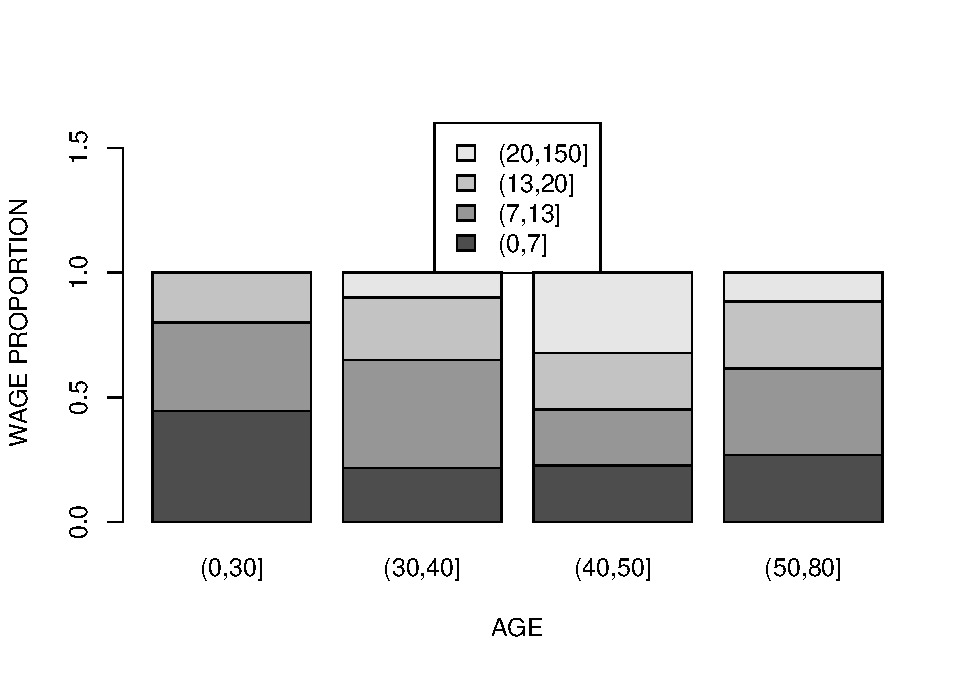
\includegraphics{Homework_3_files/figure-latex/unnamed-chunk-5-1.pdf}

\begin{enumerate}
\def\labelenumi{\alph{enumi}.}
\setcounter{enumi}{4}
\tightlist
\item
  解释:由c中的条件比例和d中的分段条形图可见,双胞胎的工资随着年龄的增长先有一定程度的提高,这可能是由于随着学历的提高和工龄的增长,双胞胎的工作能力提高,随着年龄的进步增长,工资后下降,这可能是双胞胎由于年老,工作能力下降。
\end{enumerate}


\end{document}
